\documentclass[12pt,a4paper]{report}

% ── Packages ─────────────────────────────────────────────────────────────────
\usepackage[utf8]{inputenc}
\usepackage[T1]{fontenc}
\usepackage[french]{babel}
\usepackage{geometry}
\geometry{margin=2.5cm, top=3cm, bottom=3cm}
\usepackage{lmodern}
\usepackage{microtype}
\usepackage{setspace}
\onehalfspacing

\usepackage{graphicx}
\usepackage{float}
\usepackage{amsmath, amssymb}
\usepackage{booktabs}
\usepackage{array}
\usepackage{multirow}
\usepackage{longtable}
\usepackage{xcolor}
\usepackage{colortbl}
\usepackage{tabularx}
\usepackage{hyperref}
\usepackage{fancyhdr}
\usepackage{titlesec}
\usepackage{enumitem}
\usepackage{caption}
\usepackage{subcaption}
\usepackage{listings}
\usepackage{tocloft}
\usepackage{mdframed}
\usepackage{tikz}
\usepackage{pgfplots}
\pgfplotsset{compat=1.18}

% ── Couleurs ─────────────────────────────────────────────────────────────────
\definecolor{primaryblue}{RGB}{0,70,127}
\definecolor{accentred}{RGB}{180,30,30}
\definecolor{lightgray}{RGB}{245,245,245}
\definecolor{medgray}{RGB}{200,200,200}
\definecolor{darkgray}{RGB}{80,80,80}
\definecolor{successgreen}{RGB}{30,140,60}

% ── Hyperref ─────────────────────────────────────────────────────────────────
\hypersetup{
  colorlinks=true,
  linkcolor=primaryblue,
  citecolor=accentred,
  urlcolor=primaryblue,
  pdftitle={OncoLab AI -- Rapport de Projet de Fin d'Études},
  pdfauthor={Zeroual Dhia Eddine}
}

% ── En-tête / pied de page ───────────────────────────────────────────────────
\pagestyle{fancy}
\fancyhf{}
\fancyhead[L]{\small\textcolor{primaryblue}{\textit{OncoLab AI}}}
\fancyhead[R]{\small\textcolor{darkgray}{\leftmark}}
\fancyfoot[C]{\small\thepage}
\renewcommand{\headrulewidth}{0.4pt}

% ── Style des chapitres / sections ──────────────────────────────────────────
\titleformat{\chapter}[display]
  {\normalfont\Large\bfseries\color{primaryblue}}
  {\chaptertitlename\ \thechapter}{10pt}{\Huge}
\titlespacing*{\chapter}{0pt}{30pt}{20pt}

\titleformat{\section}
  {\normalfont\large\bfseries\color{primaryblue}}
  {\thesection}{1em}{}
\titleformat{\subsection}
  {\normalfont\normalsize\bfseries\color{darkgray}}
  {\thesubsection}{1em}{}

% ── Environnement boîte ──────────────────────────────────────────────────────
\newmdenv[
  linecolor=primaryblue,
  backgroundcolor=lightgray,
  linewidth=1.2pt,
  leftmargin=0pt, rightmargin=0pt,
  innerleftmargin=10pt, innerrightmargin=10pt,
  innertopmargin=8pt, innerbottommargin=8pt
]{infobox}

% ── Style des listings ───────────────────────────────────────────────────────
\lstset{
  basicstyle=\ttfamily\small,
  backgroundcolor=\color{lightgray},
  frame=single,
  rulecolor=\color{medgray},
  breaklines=true,
  showstringspaces=false,
  keywordstyle=\color{primaryblue}\bfseries,
  commentstyle=\color{successgreen}\itshape,
  stringstyle=\color{accentred}
}

% ─────────────────────────────────────────────────────────────────────────────
\begin{document}

% ══════════════════════════════════════════════════════════════════════════════
%  PAGE DE TITRE
% ══════════════════════════════════════════════════════════════════════════════
\begin{titlepage}
\centering
\vspace*{1cm}

{\large\textcolor{darkgray}{Projet de Fin d'Études}}\\[1.5cm]

\rule{\linewidth}{1.5pt}\\[0.4cm]
{\Huge\bfseries\color{primaryblue}
  OncoLab AI\\[0.3cm]
  \large Prédiction des Complications Biologiques Induites par le FOLFOX\\
  chez les Patients Atteints de Cancer Colorectal\\
  par Apprentissage Automatique Longitudinal
}\\[0.4cm]
\rule{\linewidth}{1.5pt}\\[1.5cm]

\begin{minipage}{0.45\textwidth}
  \raggedright
  \textbf{Auteur et ML Engineer}\\
  Zeroual Dhia Eddine \\[0.4cm]
 
\end{minipage}
\hfill
\begin{minipage}{0.45\textwidth}
  \raggedleft
  \textbf{Encadrant clinique}\\
  Nadia Kerraouch\\[0.4cm]
  \textbf{Année universitaire}\\
  2025--2026\\
\end{minipage}

\vfill

\begin{infobox}
\centering
\textbf{Mots-clés :}
Cancer colorectal $\cdot$ FOLFOX $\cdot$ Apprentissage automatique longitudinal $\cdot$\\
Prédiction de toxicité $\cdot$ Méthodes d'ensemble $\cdot$ Aide à la décision clinique
\end{infobox}

\end{titlepage}

% ══════════════════════════════════════════════════════════════════════════════
%  RÉSUMÉ
% ══════════════════════════════════════════════════════════════════════════════
\chapter*{Résumé}
\addcontentsline{toc}{chapter}{Résumé}

\noindent\textbf{Contexte.}
Le cancer colorectal est l'une des maladies malignes les plus fréquentes dans le monde. Le protocole de chimiothérapie FOLFOX---combinant l'Oxaliplatine, le 5-Fluorouracile (5-FU) et l'Acide Folinique---demeure le traitement standard en contexte adjuvant et néoadjuvant, mais il induit fréquemment des toxicités biologiques sévères, notamment l'anémie, la neutropénie, la thrombocytopénie et les toxicités rénale et hépatique. L'identification précoce des patients à risque avant chaque cure permettrait un ajustement proactif des doses et réduirait les hospitalisations non programmées.

\vspace{0.5em}
\noindent\textbf{Objectif.}
Développer, valider et documenter un système d'apprentissage automatique prédisant la survenue de cinq complications induites par le FOLFOX avant chaque cure de chimiothérapie, en utilisant une représentation longitudinale des données encodant la trajectoire biologique du patient au fil des cycles successifs.

\vspace{0.5em}
\noindent\textbf{Méthodes.}
Des données cliniques réelles ont été collectées manuellement dans un seul centre : 947 enregistrements bruts provenant de 110 patients sous FOLFOX pour un cancer colorectal. Après un nettoyage rigoureux, une dédoublonnage et un encodage, des variables longitudinales ont été construites pour chaque cure, incluant les biomarqueurs décalés des un et deux cycles précédents, les variables delta (variation), les statistiques de tendance et variabilité sur 3 cycles, ainsi que des indicateurs de complications antérieures. Le jeu de données final comportait 704 cycles issus de 108 patients avec 59 variables. Quatre classifieurs d'ensemble (Random Forest, Extra Trees, XGBoost, LightGBM) ont été entraînés selon une stratégie de validation croisée sans fuite de données basée sur un découpage au niveau du patient. Un ensemble par vote souple des trois meilleurs modèles (XGBoost + LightGBM + Random Forest) a été évalué sur un ensemble de test complètement isolé de 22 patients (141 cycles) jamais vus durant l'entraînement.

\vspace{0.5em}
\noindent\textbf{Résultats.}
L'ensemble longitudinal a atteint une AUC-ROC moyenne de \textbf{0,983} sur les cinq complications. Résultats individuels : anémie AUC\,=\,0,995, sensibilité\,=\,100\,\% ; neutropénie AUC\,=\,0,954, spécificité\,=\,100\,\% ; thrombocytopénie AUC\,=\,0,993, sensibilité\,=\,100\,\% ; toxicité rénale AUC\,=\,0,999, VPP\,=\,100\,\% ; toxicité hépatique AUC\,=\,0,972, sensibilité\,=\,95,5\,\%. Les indicateurs de complications antérieures ({\tt anemia\_t1}, {\tt neutropenia\_t1}) et les biomarqueurs décalés ont été les variables les plus informatives pour toutes les cibles.

\vspace{0.5em}
\noindent\textbf{Conclusions.}
L'intégration d'un à deux cycles d'historique biologique et de statut de complication antérieur produit un outil prédictif cliniquement pertinent. Le système est reproductible, entièrement documenté et prêt pour une validation prospective. Les limites incluent le caractère rétrospectif monocentrique et la taille d'échantillon limitée pour les complications rares.

\vspace{1em}
\noindent\textbf{Mots-clés :} FOLFOX, cancer colorectal, apprentissage automatique, variables longitudinales, prédiction de toxicité, classifieur d'ensemble, aide à la décision clinique.

% ══════════════════════════════════════════════════════════════════════════════
%  TABLE DES MATIÈRES
% ══════════════════════════════════════════════════════════════════════════════
\tableofcontents
\listoffigures
\listoftables

% ══════════════════════════════════════════════════════════════════════════════
\chapter{Introduction}
% ══════════════════════════════════════════════════════════════════════════════

\section{Contexte clinique}

Le cancer colorectal (CCR) est le troisième cancer le plus fréquemment diagnostiqué et la deuxième cause de décès par cancer dans le monde. La résection chirurgicale combinée à une chimiothérapie adjuvante reste la stratégie thérapeutique principale pour les maladies localisées, tandis que la chimiothérapie néoadjuvante est de plus en plus utilisée pour réduire les tumeurs localement avancées ou rectales avant la chirurgie.

Le protocole FOLFOX---combinant l'Oxaliplatine (OXA), le 5-Fluorouracile (5-FU) et l'Acide Folinique (leucovorine)---est le schéma de chimiothérapie de première ligne standard pour le CCR en contexte adjuvant et néoadjuvant. Il est généralement administré en cycles bihebdomadaires (toutes les 14 ou 21 jours) pour un total de 8 à 12 cycles. Malgré son efficacité prouvée dans la réduction du risque de récidive et l'amélioration de la survie, le FOLFOX est associé à un large spectre de toxicités hématologiques et métaboliques pouvant compromettre la continuité du traitement et la qualité de vie des patients.

\section{Le problème clinique}

La gestion des toxicités liées au FOLFOX constitue un défi important. Les oncologues s'appuient actuellement sur les résultats biologiques obtenus à chaque visite pour détecter les complications après leur manifestation. Cette approche réactive présente plusieurs inconvénients :
\begin{itemize}
  \item Une neutropénie sévère peut ne pas être détectée avant que le patient ne présente une neutropénie fébrile, nécessitant une hospitalisation en urgence.
  \item La toxicité hématologique cumulative entraîne des réductions de doses ou des reports de cures, réduisant l'efficacité du traitement.
  \item La toxicité rénale et hépatique liée à l'Oxaliplatine peut évoluer silencieusement et ne devenir apparente qu'à des stades avancés.
  \item Il n'existe pas d'outil validé de stratification du risque permettant d'identifier, avant l'administration d'une cure, quels patients sont susceptibles de développer des complications.
\end{itemize}

Un système prédictif capable d'identifier les patients à haut risque \emph{avant} chaque cure permettrait aux oncologues d'ajuster proactivement les doses, de planifier une surveillance renforcée, de prescrire un traitement de soutien (ex. G-CSF pour la neutropénie, agents stimulants l'érythropoïèse pour l'anémie) ou de reporter la cure jusqu'à l'amélioration des paramètres biologiques du patient.

\section{Pourquoi des variables longitudinales ?}

L'hypothèse centrale de ce travail est qu'une \emph{seule} valeur de bilan biologique est un faible prédicteur des complications à venir. L'intuition clinique, confirmée par les données, suggère que la trajectoire importe bien plus que la photo instantanée :

\begin{infobox}
Un patient avec une hémoglobine de 10,5\,g/dL stable depuis trois cycles présente un profil de risque très différent d'un patient dont l'hémoglobine était de 13,0\,g/dL il y a deux cycles et qui chute rapidement. Les deux patients ont la même valeur actuelle ; seul le modèle longitudinal peut les distinguer.
\end{infobox}

En encodant l'historique biologique de chaque patient sous forme de variables numériques concrètes (valeurs décalées, variations delta, tendances multi-cycles), le modèle capture la \emph{direction}, la \emph{vitesse} et la \emph{volatilité} de la détérioration---précisément les signaux qu'un oncologue expérimenté utilise en consultant le dossier d'un patient.

\section{Objectifs du projet}

Ce projet poursuit quatre objectifs interdépendants :
\begin{enumerate}
  \item \textbf{Pipeline de données :} construire un pipeline entièrement reproductible et documenté transformant une feuille de calcul clinique brute en un jeu de données longitudinal prêt pour l'apprentissage automatique.
  \item \textbf{Ingénierie des variables :} concevoir et valider un ensemble de variables longitudinales encodant la trajectoire du patient au fil des cycles FOLFOX successifs.
  \item \textbf{Développement du modèle :} entraîner et évaluer des classifieurs d'ensemble avec une stratégie de validation croisée sans fuite de données, basée sur un découpage au niveau du patient.
  \item \textbf{Livrables cliniques :} produire un tableau de prédictions par patient, des artefacts de modèles entraînés et une documentation complète pour un usage clinique et une validation prospective.
\end{enumerate}

\section{Contributions}

Les principales contributions de ce travail sont :
\begin{itemize}
  \item Un notebook de préparation des données complet et open-source ({\tt 1\_data\_preparation.ipynb}) traitant tous les problèmes de qualité de données réels présents dans la collecte clinique brute.
  \item Une représentation longitudinale originale des variables pour les cycles FOLFOX, incluant les biomarqueurs décalés, les variables delta, les statistiques de tendance et variabilité sur 3 cycles, et les indicateurs de complications antérieures.
  \item Un système d'ensemble atteignant une AUC-ROC moyenne de 0,983 sur cinq complications sur une cohorte de test indépendante.
  \item Un tableau de prédictions par patient permettant une vérification clinique directe.
  \item Un dictionnaire de données entièrement documenté couvrant les 59 variables.
\end{itemize}

\section{Structure du rapport}

Le chapitre~\ref{chap:background} présente le contexte clinique et technique. Le chapitre~\ref{chap:related} passe en revue les travaux connexes. Le chapitre~\ref{chap:data} décrit en détail le pipeline de collecte, nettoyage et ingénierie des données. Le chapitre~\ref{chap:methodology} présente la méthodologie de modélisation et la stratégie de validation. Le chapitre~\ref{chap:results} présente l'ensemble des résultats expérimentaux. Le chapitre~\ref{chap:discussion} discute des implications cliniques, des limites et des perspectives. Le chapitre~\ref{chap:conclusion} conclut.

% ══════════════════════════════════════════════════════════════════════════════
\chapter{Contexte clinique et technique}
\label{chap:background}
% ══════════════════════════════════════════════════════════════════════════════

\section{Le cancer colorectal}

Le cancer colorectal se développe à partir de l'épithélium de la muqueuse du côlon ou du rectum. La grande majorité (>95\,\%) sont des adénocarcinomes. La stadification est réalisée selon la classification TNM :
\begin{itemize}
  \item \textbf{T} (tumeur) : étendue de l'invasion tumorale primaire (T0--T4).
  \item \textbf{N} (nœuds) : présence et étendue de l'atteinte ganglionnaire régionale (N0--N2).
  \item \textbf{M} (métastase) : présence de métastases à distance (M0 ou M1).
\end{itemize}
Le stade détermine le pronostic et guide le choix thérapeutique. Les patients de stade III (T1--4, N1--2, M0) sont candidats au FOLFOX adjuvant. Les patients de stade IV (tout T, tout N, M1) reçoivent généralement le FOLFOX en première ligne de traitement palliatif.

\section{Le protocole FOLFOX}

Le FOLFOX est administré selon un protocole de perfusion bihebdomadaire. Le schéma standard (FOLFOX4/FOLFOX6) comprend :
\begin{itemize}
  \item \textbf{Oxaliplatine} (85\,mg/m² en 2 heures) : un composé platinique formant des adduits d'ADN conduisant à l'arrêt de la réplication. Toxicités principales : neuropathie périphérique, myélosuppression.
  \item \textbf{5-FU bolus} (400\,mg/m²) + \textbf{5-FU en perfusion continue} (2400\,mg/m² sur 46 heures) : un antimétabolite fluoropyrimidine. Toxicités principales : mucite, myélosuppression, hépatotoxicité.
  \item \textbf{Acide folinique (leucovorine)} (400\,mg/m²) : potentialise l'activité du 5-FU.
\end{itemize}

En pratique clinique, des réductions de doses (généralement 20--25\,\%) ou des reports de cures sont appliqués lors de la détection d'une toxicité significative. Ces modifications sont associées à de moins bons résultats oncologiques.

\section{Les complications biologiques induites par le FOLFOX}

Ce projet prédit cinq complications binaires, définies à chaque cure selon les seuils cliniques utilisés dans la collecte originale des données :

\begin{table}[H]
\centering
\caption{Complications biologiques du FOLFOX et seuils cliniques}
\label{tab:complications}
\begin{tabular}{lllr}
\toprule
\textbf{Complication} & \textbf{Biomarqueur} & \textbf{Seuil} & \textbf{Prévalence} \\
\midrule
Anémie & Hémoglobine (Hb) & En dessous de la norme pour le sexe & 68,0\,\% \\
Neutropénie & Numération des neutrophiles & $< 1,5$\,G/L & 5,1\,\% \\
Thrombocytopénie & Numération plaquettaire & $< 150$\,G/L & 17,9\,\% \\
Toxicité rénale & Créatinine / Urée & Valeurs élevées & 9,1\,\% \\
Toxicité hépatique & ASAT, ALAT & $> 3\times$ limite supérieure de la normale & 28,6\,\% \\
\bottomrule
\end{tabular}
\end{table}

Les prévalences du tableau~\ref{tab:complications} sont calculées au niveau des cycles sur les 704 cycles du jeu de données longitudinal. L'anémie est la plus fréquente (68\,\%) car le seuil est inclusif des anémies légères et le FOLFOX est connu pour provoquer une toxicité hématologique progressive. La neutropénie est la plus rare (5,1\,\%) et cliniquement la plus dangereuse, une neutropénie de grade 4 pouvant mettre la vie en danger.

\section{L'apprentissage automatique pour l'aide à la décision clinique}

Les systèmes d'aide à la décision clinique (SADC) basés sur l'apprentissage automatique visent à augmenter, et non à remplacer, le jugement médical. En oncologie, l'apprentissage automatique a été appliqué à :
\begin{itemize}
  \item \textbf{La prédiction de la survie :} estimation de la survie globale et sans progression.
  \item \textbf{L'optimisation des doses :} recommandation d'ajustements de doses basés sur le risque de toxicité prédit.
  \item \textbf{La prédiction de la toxicité :} identification des patients à haut risque d'effets indésirables spécifiques.
  \item \textbf{La prédiction de la récidive :} estimation du risque de récurrence après chirurgie.
\end{itemize}

Pour la prédiction de toxicité spécifiquement, les défis principaux sont le déséquilibre de classes (événements rares comme la neutropénie), la dépendance temporelle (chaque cycle dépend de l'historique du patient) et la fuite de données (les informations du test ne doivent pas influencer le processus d'entraînement).

% ══════════════════════════════════════════════════════════════════════════════
\chapter{Travaux connexes}
\label{chap:related}
% ══════════════════════════════════════════════════════════════════════════════

\section{Apprentissage automatique pour la prédiction de la toxicité chimiothérapeutique}

Plusieurs études ont appliqué l'apprentissage automatique à la prédiction d'effets indésirables liés à la chimiothérapie, bien que peu se concentrent spécifiquement sur le FOLFOX dans le cancer colorectal :

\begin{itemize}
  \item \textbf{Les approches transversales} utilisent des variables provenant d'un seul point dans le temps (ex. caractéristiques de base du patient et valeurs biologiques pré-cure). Bien que ces modèles soient plus faciles à construire, ils ne peuvent pas capturer la détérioration dynamique des paramètres hématologiques d'un patient au fil des cycles successifs.
  \item \textbf{Les approches longitudinales} intègrent des séquences temporelles de mesures, soit par ingénierie explicite des variables (valeurs décalées, delta, tendances), soit par des modèles de séquences (LSTM, Transformer). Ces approches surpassent généralement les baselines transversales lorsqu'un historique suffisant est disponible.
  \item \textbf{Les méthodes d'ensemble} (Random Forest, XGBoost, LightGBM) surpassent systématiquement les classifieurs uniques sur les données cliniques tabulaires, grâce à leur robustesse au bruit et leur capacité à gérer des types de variables mixtes sans prétraitement extensif.
\end{itemize}

\section{Considérations méthodologiques clés}

Les études dans ce domaine souffrent fréquemment de défauts méthodologiques qui gonflent les performances rapportées :
\begin{enumerate}
  \item \textbf{Fuite au niveau du patient :} découper le train/test par ligne (ignorant l'identité du patient) permet à plusieurs lignes du même patient d'apparaître à la fois dans le train et le test, augmentant artificiellement les métriques.
  \item \textbf{Fuite de mise à l'échelle des variables :} ajuster le \texttt{StandardScaler} sur l'ensemble des données (avant la validation croisée) fait fuir les statistiques de distribution du jeu de validation dans le processus d'entraînement.
  \item \textbf{Absence d'ordre temporel :} une validation croisée ignorant le temps peut entraîner sur des cycles futurs et prédire des cycles passés, ce qui est impossible en déploiement.
\end{enumerate}

Ce projet traite explicitement ces trois problèmes, comme décrit au chapitre~\ref{chap:methodology}.

\section{Positionnement de ce travail}

Ce travail occupe une niche spécifique : un jeu de données FOLFOX réel, monocentrique, de taille modeste (108 patients), avec un accent sur la transparence rigoureuse du pipeline et la reproductibilité. Contrairement à de nombreuses études publiées, le notebook complet de préparation des données, la logique d'ingénierie des variables et les artefacts de modèles entraînés sont fournis comme livrables. L'approche d'ingénierie des variables longitudinales constitue la contribution méthodologique principale.

% ══════════════════════════════════════════════════════════════════════════════
\chapter{Données}
\label{chap:data}
% ══════════════════════════════════════════════════════════════════════════════

\section{Collecte des données}

\subsection{Source}
Le jeu de données brut a été fourni par l'encadrant clinique. Les données ont été collectées manuellement à partir des dossiers des patients dans un seul centre d'oncologie. Chaque ligne de la feuille de calcul brute correspond à une cure de chimiothérapie pour un patient. Les données ont été enregistrées dans un document Google Sheets et exportées sous forme de fichier CSV nommé \texttt{Collect Data Onco Lab AI - Feuille 2.csv}.

\subsection{Caractéristiques du jeu de données brut}
\begin{itemize}
  \item \textbf{Taille :} 947 lignes $\times$ 42 colonnes
  \item \textbf{Patients :} 110 identifiants de patients uniques (bruts)
  \item \textbf{Format :} en-têtes de colonnes en français ; format décimal européen (séparateur virgule) ; chaînes structurées pour les champs de cure et de stadification
  \item \textbf{Période :} plusieurs cycles par patient ; les cures vont de C0 à C17
\end{itemize}

\section{Pipeline de nettoyage des données}

Le pipeline complet de nettoyage est implémenté dans \texttt{notebooks/1\_data\_preparation.ipynb}. Le tableau~\ref{tab:cleaning} résume les principaux problèmes identifiés et les résolutions appliquées.

\begin{table}[H]
\centering
\caption{Problèmes de qualité des données et résolutions}
\label{tab:cleaning}
\begin{tabular}{p{4cm}p{5cm}p{5cm}}
\toprule
\textbf{Problème} & \textbf{Données affectées} & \textbf{Résolution} \\
\midrule
En-têtes en français & Les 42 colonnes & Renommées en snake\_case anglais \\
Format décimal européen (\texttt{"11,7"}) & Toutes les colonnes numériques & Remplacement virgule $\to$ point ; conversion en flottant \\
Doublons (patient, cure) & 26 lignes supprimées sur 20 patients & Conserver la dernière ligne (la cure administrée) \\
Casse de l'identifiant patient (\texttt{p16} vs \texttt{P16}) & 1 patient & Mise en majuscules de tous les identifiants \\
Corruption de la chaîne TNM & Patient P31 (toutes les cures) & Forçage du stade correct \texttt{T3N1M0} \\
\texttt{Stade 4} sans chiffre M & Patient P107 & Définir \texttt{M\_stage = 1} (stade IV implique M1) \\
Erreur de saisie : \texttt{uree = 36} & 1 ligne & Corrigé à 0,36 g/L (erreur de virgule décimale) \\
Biomarqueurs en cellules/µL & \texttt{plq}, \texttt{neut} et colonnes dérivées & Division par 1000 pour obtenir G/L \\
\bottomrule
\end{tabular}
\end{table}

\subsection{Renommage des colonnes et encodage}

Les en-têtes français ont été mappés vers des identifiants anglais en snake\_case (ex. \textit{Anémie} $\to$ \texttt{anemia}, \textit{Toxicité hépatique} $\to$ \texttt{hepatic\_toxicity}). Les variables catégorielles ont été normalisées :
\begin{itemize}
  \item \textbf{Etat} (statut nutritionnel) : 12 variantes brutes regroupées en \texttt{Sous-poids} / \texttt{Normale} / \texttt{Surpoids}.
  \item \textbf{Adj/Néoadj} : 4 variantes brutes (\texttt{adj}, \texttt{AdJ}, \texttt{Adj}, \texttt{Neoadj}) normalisées en \texttt{Adj} / \texttt{Neoadj}.
  \item \textbf{Sexe} : \texttt{H}/\texttt{F} $\to$ binaire \texttt{sex\_M} (1\,=\,masculin).
\end{itemize}

Les chaînes structurées ont été analysées :
\begin{itemize}
  \item \texttt{Cure} (ex. \texttt{"C3"}) $\to$ entier \texttt{cycle\_num}
  \item \texttt{Intervalle} (ex. \texttt{"15J"}) $\to$ entier \texttt{interval\_days}
  \item \texttt{Stade} (ex. \texttt{"T3N1M0"}) $\to$ entiers \texttt{T\_stage}, \texttt{N\_stage}, \texttt{M\_stage}
\end{itemize}

\subsection{Dédoublonnage}

Vingt patients avaient plusieurs lignes pour la même cure. Après investigation, cela correspond à des événements de reprogrammation : une cure initialement reportée ou interrompue a été enregistrée deux fois---une fois avec des données partielles et une fois pour la cure effectivement administrée. Les lignes ont été triées par (\texttt{patient\_id}, \texttt{cycle\_num}) en préservant l'ordre original du CSV pour les égalités, puis dédoublonnées en conservant la dernière ligne (la cure administrée). Cela a réduit le jeu de données de 947 à 921 lignes.

\section{Description de la cohorte de patients}

\begin{table}[H]
\centering
\caption{Résumé de la cohorte de patients (108 patients, 704 cycles)}
\label{tab:cohort}
\begin{tabular}{llr}
\toprule
\textbf{Caractéristique} & \textbf{Catégorie / Statistique} & \textbf{Valeur} \\
\midrule
\multirow{3}{*}{Âge (années)} & Moyenne $\pm$ ET & $57{,}6 \pm 12{,}1$ \\
 & Étendue & 26--83 \\
\midrule
\multirow{2}{*}{Sexe} & Masculin & 78 (72,2\,\%) \\
 & Féminin & 30 (27,8\,\%) \\
\midrule
IMC (kg/m²) & Moyenne $\pm$ ET & $23{,}5 \pm 4{,}0$ \\
\midrule
\multirow{3}{*}{Cures par patient} & Moyenne & 6,5 \\
 & Médiane & 6 \\
 & Étendue & 1--11 (après dédoublonnage) \\
\midrule
\multirow{2}{*}{Intention du traitement} & Adjuvant & 72 (66,7\,\%) \\
 & Néoadjuvant & 36 (33,3\,\%) \\
\midrule
\multirow{2}{*}{Maladie métastatique} & Non & 80 (74,1\,\%) \\
 & Oui & 28 (25,9\,\%) \\
\midrule
\multirow{4}{*}{Stade T} & T1 & 3 (2,8\,\%) \\
 & T2 & 21 (19,4\,\%) \\
 & T3 & 72 (66,7\,\%) \\
 & T4 & 11 (10,2\,\%) \\
\midrule
\multirow{3}{*}{Stade N} & N0 & 9 (8,3\,\%) \\
 & N1 & 60 (55,6\,\%) \\
 & N2 & 38 (35,2\,\%) \\
\midrule
\multirow{4}{*}{Comorbidités} & Hypertension artérielle & 56 (51,9\,\%) \\
 & Diabète & 59 (54,6\,\%) \\
 & Maladie rénale chronique & 5 (4,6\,\%) \\
 & Maladie hépatique chronique & 4 (3,7\,\%) \\
\midrule
\multirow{3}{*}{Localisation du cancer} & Côlon (tous types) & 94 (87,0\,\%) \\
 & Rectum (tous types) & 13 (12,0\,\%) \\
 & Côlon + péritoine & 1 (0,9\,\%) \\
\bottomrule
\end{tabular}
\end{table}

La cohorte est majoritairement masculine (72\,\%), avec un âge moyen de 57,6 ans. La maladie T3 (66,7\,\%) et l'atteinte ganglionnaire N1 (55,6\,\%) sont les catégories de stadification les plus fréquentes, cohérentes avec la distribution attendue des patients CCR traités par FOLFOX. Les comorbidités métaboliques (diabète 54,6\,\%, hypertension 51,9\,\%) sont très prévalentes, reflétant le profil d'âge de la cohorte.

\section{Valeurs biologiques de base}

Le tableau~\ref{tab:bio} résume la distribution des huit biomarqueurs de la cure en cours sur l'ensemble des 704 cycles.

\begin{table}[H]
\centering
\caption{Distribution des biomarqueurs sur tous les cycles (après corrections d'unités)}
\label{tab:bio}
\begin{tabular}{llrrrr}
\toprule
\textbf{Biomarqueur} & \textbf{Unité} & \textbf{Moyenne} & \textbf{ET} & \textbf{Min} & \textbf{Max} \\
\midrule
Hémoglobine (Hb) & g/dL & 11,63 & 1,52 & 6,60 & 16,20 \\
Neutrophiles (Neut) & G/L & 4,16 & 1,85 & 0,70 & 11,40 \\
Plaquettes (Plq) & G/L & 212,5 & 78,5 & 6,72 & 596,0 \\
Urée & g/L & 0,34 & -- & 0,10 & 0,45$^{*}$ \\
Créatinine & mg/L & 9,10 & 2,15 & 3,50 & 29,0 \\
ASAT & UI/L & 26,8 & 16,3 & 5,0 & 163,0 \\
ALAT & UI/L & 24,6 & 15,3 & 1,0 & 144,0 \\
Bilirubine totale & mg/L & 5,91 & 3,76 & 1,0 & 60,4 \\
\bottomrule
\multicolumn{6}{l}{\small $^{*}$ Après correction d'une saisie erronée (36 g/L $\to$ 0,36 g/L).}
\end{tabular}
\end{table}

La valeur moyenne d'Hb de 11,63\,g/dL est inférieure à la normale pour les deux sexes, cohérente avec la forte prévalence de l'anémie. Les numérations plaquettaires présentent une variance élevée, avec un minimum de 6,72\,G/L indiquant une thrombocytopénie sévère dans certains cycles.

\section{Ingénierie des variables longitudinales}
\label{sec:features}

Toutes les variables sont calculées au sein de l'historique chronologique de chaque patient à l'aide d'opérations \texttt{groupby(\textquotesingle patient\_id\textquotesingle)} après tri par \texttt{cycle\_num}. L'utilisation de valeurs provenant de cycles futurs constituerait une fuite de données et est explicitement évitée.

\subsection{Biomarqueurs décalés}

Pour quatre biomarqueurs clés (Hb, neutrophiles, plaquettes, créatinine), les valeurs des un et deux cycles précédents sont ajoutées comme variables explicites :
\begin{align}
  x^{(t-1)}_{\text{col}} &= \texttt{shift}(1) \text{ au sein du groupe patient} \\
  x^{(t-2)}_{\text{col}} &= \texttt{shift}(2) \text{ au sein du groupe patient}
\end{align}
Cela produit 8 variables supplémentaires : \texttt{hb\_t1}, \texttt{neut\_t1}, \texttt{plq\_t1}, \texttt{creat\_t1} et leurs homologues \texttt{\_t2}.

\subsection{Indicateurs de complications antérieures}

Pour chacune des cinq complications, des indicateurs binaires signalant si la complication est survenue lors du cycle précédent (t-1) ou deux cycles auparavant (t-2) sont ajoutés :
\begin{align}
  \texttt{anemia\_t1} &= \texttt{shift}(1)[\texttt{target\_anemia}]
\end{align}
Cela produit 10 variables (\texttt{anemia\_t1}, \ldots, \texttt{hepatic\_toxicity\_t2}) encodant le signal de récidive, cliniquement reconnu comme fort pour les toxicités du FOLFOX.

\subsection{Variables delta}

La variation absolue d'un biomarqueur par rapport au cycle précédent capture la vitesse et la direction de la détérioration biologique :
\begin{align}
  \texttt{delta\_hb}   &= \texttt{hb}   - \texttt{hb\_t1} \\
  \texttt{delta\_neut} &= \texttt{neut} - \texttt{neut\_t1} \\
  \texttt{delta\_plq}  &= \texttt{plq}  - \texttt{plq\_t1}
\end{align}
Un \texttt{delta\_hb} négatif indique une chute de l'hémoglobine---une trajectoire vers l'anémie même si la valeur absolue actuelle reste dans une fourchette acceptable.

\subsection{Variables de tendance et de variabilité}

Les dynamiques multi-cycles sont capturées par trois statistiques sommaires calculées sur une fenêtre de 3 cycles :
\begin{align}
  \texttt{trend\_neut\_3cycles} &= \frac{\texttt{neut\_t2} + \texttt{neut\_t1} + \texttt{neut}}{3} \\
  \texttt{variability\_neut}    &= \text{ET}(\texttt{neut\_t2},\ \texttt{neut\_t1},\ \texttt{neut}) \\
  \texttt{drop\_rate\_plq}      &= \frac{\texttt{plq} - \texttt{plq\_t2}}{\texttt{plq\_t2}}
\end{align}
\texttt{drop\_rate\_plq} est sans dimension (un ratio de numérations plaquettaires dans la même unité), donc aucune correction d'unité n'est nécessaire malgré la conversion cells/µL $\to$ G/L appliquée aux valeurs absolues.

\subsection{Filtrage des lignes}

Les lignes où les variables de décalage \texttt{\_t2} sont NaN (cycles 1 et 2 de chaque patient, sans historique sur deux cycles) sont supprimées. Cela réduit le jeu de données de 921 à \textbf{704 lignes} (108 patients), une réduction d'environ 23,5\,\%, entièrement attendue.

\subsection{Récapitulatif des groupes de variables}

\begin{table}[H]
\centering
\caption{Groupes de variables dans le jeu de données longitudinal}
\label{tab:features}
\begin{tabular}{lp{5cm}r}
\toprule
\textbf{Groupe} & \textbf{Colonnes} & \textbf{Nombre} \\
\midrule
Démographie patient & age, sex\_M, bmi, etat, comorbidity\_count & 5 \\
Comorbidités (binaires) & hta, diabetes, renal\_disease, hepatic\_disease & 4 \\
Stadification du cancer & cancer\_type, T\_stage, N\_stage, M\_stage, has\_metastasis, treatment\_intent & 6 \\
Paramètres de cure & cycle\_num, interval\_days & 2 \\
Doses & dose\_oxali, dose\_5fu\_bolus, dose\_5fu\_cont, dose\_af & 4 \\
Biomarqueurs actuels & hb, neut, plq, uree, creat, asat, alat, bil & 8 \\
Biomarqueurs décalés (t-1) & hb\_t1, neut\_t1, plq\_t1, creat\_t1 & 4 \\
Biomarqueurs décalés (t-2) & hb\_t2, neut\_t2, plq\_t2, creat\_t2 & 4 \\
Complications antérieures (t-1) & anemia\_t1, \ldots, hepatic\_toxicity\_t1 & 5 \\
Complications antérieures (t-2) & anemia\_t2, \ldots, hepatic\_toxicity\_t2 & 5 \\
Variables delta & delta\_hb, delta\_neut, delta\_plq & 3 \\
Tendance / variabilité & trend\_neut\_3cycles, drop\_rate\_plq, variability\_neut & 3 \\
\textbf{Cibles} & target\_anemia, \ldots, target\_hepatic\_toxicity & 5 \\
\midrule
\textbf{Total (variables uniquement)} & & \textbf{54} \\
\textbf{Total (variables + cibles)} & & \textbf{59} \\
\bottomrule
\end{tabular}
\end{table}

\section{Distribution des cibles et déséquilibre de classes}

\begin{table}[H]
\centering
\caption{Prévalence des complications dans le jeu de données longitudinal}
\label{tab:imbalance}
\begin{tabular}{lrrl}
\toprule
\textbf{Cible} & \textbf{Cycles positifs} & \textbf{Total cycles} & \textbf{Prévalence} \\
\midrule
Anémie & 479 & 704 & 68,0\,\% \\
Toxicité hépatique & 201 & 704 & 28,6\,\% \\
Thrombocytopénie & 126 & 704 & 17,9\,\% \\
Toxicité rénale & 64 & 704 & 9,1\,\% \\
\textbf{Neutropénie} & \textbf{36} & \textbf{704} & \textbf{5,1\,\%} \\
\bottomrule
\end{tabular}
\end{table}

Le jeu de données présente un déséquilibre de classes sévère, particulièrement pour la neutropénie (5,1\,\%). Cela nécessite un traitement spécifique lors de l'entraînement du modèle : les modèles à base de forêts utilisent \texttt{class\_weight=\textquotesingle{}balanced\textquotesingle{}}, tandis que XGBoost utilise \texttt{scale\_pos\_weight = N\_neg / N\_pos}. L'AUC-ROC est utilisée comme métrique d'évaluation principale car elle est insensible au déséquilibre de classes par conception.

% ══════════════════════════════════════════════════════════════════════════════
\chapter{Méthodologie}
\label{chap:methodology}
% ══════════════════════════════════════════════════════════════════════════════

\section{Formulation du problème}

Le problème est formulé comme cinq tâches indépendantes de classification binaire. Pour chaque complication $c \in \{\text{anémie, neutropénie, thrombocytopénie, rénale, hépatique}\}$ et chaque cycle $t$, le modèle prédit :
\[
\hat{y}_t^{(c)} = f_c\!\left(x_t,\; x_{t-1},\; x_{t-2}\right) \in [0, 1]
\]
où $x_t$ est le vecteur de variables au cycle $t$ (biomarqueurs actuels, dose, démographie), et $x_{t-1}$, $x_{t-2}$ représentent l'historique encodé dans les variables décalées, delta, tendance et indicateurs de complications antérieures. La sortie est une probabilité que la complication $c$ soit observée après le cycle $t$.

\section{Prévention de la fuite de données}
\label{sec:leakage}

Deux sources de fuite sont explicitement éliminées :

\subsection{Fuite au niveau du patient}

Dans un jeu de données cliniques longitudinal, plusieurs lignes appartiennent au même patient. Un découpage naïf train/test par ligne permet au modèle de s'entraîner sur les cycles 1 à 5 d'un patient et de tester sur le cycle 6 du \emph{même} patient. Le modèle peut alors identifier implicitement la trajectoire du patient et « tricher », produisant des estimations de performance optimistes qui ne se généralisent pas.

\textbf{Solution :} tous les découpages utilisent \texttt{GroupShuffleSplit} et \texttt{GroupKFold} avec \texttt{groups = patient\_id}. Cela garantit qu'aucun patient n'apparaît à la fois dans l'entraînement et la validation (ou le test) à aucune étape.

\subsection{Fuite de mise à l'échelle des variables}

Ajuster le \texttt{StandardScaler} sur l'ensemble combiné entraînement + validation avant la validation croisée fait fuir les statistiques de distribution du jeu de validation dans le processus d'entraînement.

\textbf{Solution :} au sein de chaque pli de la validation croisée, un nouveau \texttt{StandardScaler} est ajusté \emph{uniquement} sur les lignes d'entraînement du pli, puis appliqué à la fois aux lignes d'entraînement et de validation du pli. L'ensemble de test n'est jamais touché par aucun normalisateur pendant la validation croisée.

\section{Stratégie de validation}

\begin{figure}[H]
\centering
\begin{tikzpicture}[node distance=0.4cm and 0.3cm, font=\small]
  \draw[primaryblue, thick] (0,0) rectangle (12,1.2);
  \node[primaryblue] at (6,0.9) {\footnotesize 704 lignes $\cdot$ 108 patients};
  \draw[successgreen, thick, fill=successgreen!10] (0.1,0.1) rectangle (9.5,0.75);
  \node[successgreen] at (4.8,0.42) {ENTRAÎNEMENT -- 86 patients / 563 lignes};
  \draw[accentred, thick, fill=accentred!10] (9.6,0.1) rectangle (11.9,0.75);
  \node[accentred] at (10.75,0.42) {TEST};
  \node[below] at (10.75,0.05) {\footnotesize 22 pat. / 141 lignes};
  \node[below] at (4.8,0.0) {\footnotesize GroupShuffleSplit(test\_size=0,20, random\_state=42)};
\end{tikzpicture}
\vspace{0.5em}

\begin{tikzpicture}[node distance=0.3cm, font=\small]
  \foreach \i/\c in {0/primaryblue!30, 1/primaryblue!30, 2/primaryblue!30, 3/primaryblue!30, 4/accentred!25} {
    \pgfmathsetmacro{\x}{\i * 2.3}
    \draw[\c, thick, fill=\c] (\x, 0) rectangle (\x+2.2, 0.7);
  }
  \node at (0*2.3+1.1, 0.35) {\footnotesize Entr.};
  \node at (1*2.3+1.1, 0.35) {\footnotesize Entr.};
  \node at (2*2.3+1.1, 0.35) {\footnotesize Entr.};
  \node at (3*2.3+1.1, 0.35) {\footnotesize Entr.};
  \node[accentred] at (4*2.3+1.1, 0.35) {\footnotesize \textbf{Val.}};
  \node[below] at (5.75, -0.1) {\footnotesize GroupKFold (5 plis) $\times$ 5 rotations $\to$ AUC moyenne par modèle};
\end{tikzpicture}
\caption{Stratégie de validation : découpage 80/20 au niveau du patient suivi d'une validation croisée GroupKFold à 5 plis sur l'ensemble d'entraînement.}
\label{fig:cv}
\end{figure}

L'ensemble d'entraînement (86 patients, 563 cycles) est utilisé pour toute la validation croisée et la sélection de modèle. L'ensemble de test (22 patients, 141 cycles) est complètement isolé et n'est évalué qu'une seule fois, à la fin.

\section{Modèles}

Quatre classifieurs d'ensemble ont été évalués :

\begin{table}[H]
\centering
\caption{Modèles et hyperparamètres}
\label{tab:models}
\begin{tabular}{llp{5.5cm}}
\toprule
\textbf{Modèle} & \textbf{Bibliothèque} & \textbf{Paramètres clés} \\
\midrule
Random Forest & scikit-learn & 300 arbres, \texttt{class\_weight=\textquotesingle{}balanced\textquotesingle{}} \\
Extra Trees & scikit-learn & 300 arbres, \texttt{class\_weight=\textquotesingle{}balanced\textquotesingle{}} \\
XGBoost & xgboost & 300 itérations, \texttt{max\_depth=4}, \texttt{lr=0,05}, \texttt{scale\_pos\_weight=neg/pos} \\
LightGBM & lightgbm & 300 itérations, \texttt{max\_depth=4}, \texttt{lr=0,05}, \texttt{class\_weight=\textquotesingle{}balanced\textquotesingle{}} \\
\bottomrule
\end{tabular}
\end{table}

Au sein de chaque pli de validation croisée, un clone de l'estimateur (\texttt{sklearn.base.clone}) est entraîné pour éviter l'accumulation d'état entre les plis.

\section{Construction de l'ensemble (vote souple)}

Après la validation croisée, les trois modèles avec la plus haute \emph{AUC-ROC CV moyenne sur les cinq cibles} sont sélectionnés comme membres de l'ensemble. La sélection est effectuée uniquement sur les résultats de validation croisée---l'ensemble de test n'est jamais consulté. Les modèles sélectionnés sont ensuite réentraînés sur l'\emph{ensemble complet} d'entraînement, et leurs probabilités prédites sont moyennées (vote souple) :
\[
\hat{p}_{\text{ens}} = \frac{1}{3} \sum_{k=1}^{3} \hat{p}_k
\]

La moyenne des probabilités préserve l'information de confiance et surpasse les ensembles à vote majoritaire dur pour les classifieurs calibrés.

Dans cette expérience, les 3 meilleurs modèles par AUC CV moyenne étaient :
\begin{center}
\textbf{XGBoost (0,9767)} $\approx$ \textbf{LightGBM (0,9756)} $\approx$ \textbf{Random Forest (0,9750)}
\end{center}
Extra Trees (AUC CV moyenne\,=\,0,938) a été exclu de l'ensemble.

\section{Métriques d'évaluation}

Pour chaque cible indépendamment, les métriques suivantes sont calculées sur l'ensemble de test isolé :
\begin{itemize}
  \item \textbf{AUC-ROC} : aire sous la courbe ROC. Indépendante du seuil ; adaptée aux classes déséquilibrées. Métrique principale.
  \item \textbf{Sensibilité (Rappel)} : $\text{VP} / (\text{VP} + \text{FN})$. Proportion des complications réelles détectées. Cliniquement la plus importante---une complication manquée est plus dangereuse qu'une fausse alarme.
  \item \textbf{Spécificité} : $\text{VN} / (\text{VN} + \text{FP})$. Proportion des non-événements correctement identifiés comme négatifs.
  \item \textbf{VPP (Précision)} : $\text{VP} / (\text{VP} + \text{FP})$. Quand le modèle signale un patient, à quelle fréquence a-t-il raison ?
  \item \textbf{Score F1} : moyenne harmonique de la sensibilité et de la VPP. Résumé équilibré pour les classes déséquilibrées.
\end{itemize}
Les prédictions binaires sont produites à un seuil de 0,50 appliqué aux probabilités de l'ensemble.

\section{Importance des variables}

L'importance des variables post-hoc est calculée en utilisant la Diminution Moyenne de l'Impureté (DMI) du Random Forest, entraîné sur l'ensemble complet d'entraînement. La DMI mesure de combien chaque variable réduit l'impureté (Gini) sur tous les arbres, en moyenne.

% ══════════════════════════════════════════════════════════════════════════════
\chapter{Résultats}
\label{chap:results}
% ══════════════════════════════════════════════════════════════════════════════

\section{Résultats de la validation croisée}

Le tableau~\ref{tab:cv} rapporte l'AUC-ROC de la validation croisée GroupKFold à 5 plis sur l'ensemble d'entraînement (moyenne $\pm$ écart-type sur les plis). Les plis où l'ensemble de validation ne contenait qu'une seule classe sont exclus du calcul de l'AUC.

\begin{table}[H]
\centering
\caption{AUC-ROC de la validation croisée GroupKFold à 5 plis (ensemble d'entraînement, moyenne ± ET)}
\label{tab:cv}
\setlength{\tabcolsep}{4pt}
\begin{tabular}{lccccc}
\toprule
\textbf{Modèle} & \textbf{Anémie} & \textbf{Neutropénie} & \textbf{Thrombocy.} & \textbf{Rénale} & \textbf{Hépatique} \\
\midrule
Random Forest & $0{,}969 \pm 0{,}012$ & $0{,}976 \pm 0{,}036$ & $0{,}995 \pm 0{,}002$ & $0{,}952 \pm 0{,}086$ & $0{,}983 \pm 0{,}015$ \\
Extra Trees   & $0{,}964 \pm 0{,}009$ & $0{,}909 \pm 0{,}090$ & $0{,}977 \pm 0{,}010$ & $0{,}928 \pm 0{,}089$ & $0{,}913 \pm 0{,}025$ \\
XGBoost       & $0{,}979 \pm 0{,}011$ & $0{,}993 \pm 0{,}012$ & $0{,}997 \pm 0{,}003$ & $0{,}930 \pm 0{,}094$ & $0{,}984 \pm 0{,}011$ \\
LightGBM      & $0{,}980 \pm 0{,}013$ & $0{,}996 \pm 0{,}008$ & $0{,}997 \pm 0{,}002$ & $0{,}923 \pm 0{,}102$ & $0{,}983 \pm 0{,}014$ \\
\midrule
\textbf{Moyenne} & & & & & \\
Random Forest & \multicolumn{5}{c}{0,9750 $\leftarrow$ \textbf{dans l'ensemble}} \\
Extra Trees   & \multicolumn{5}{c}{0,9383} \\
XGBoost       & \multicolumn{5}{c}{0,9767 $\leftarrow$ \textbf{dans l'ensemble}} \\
LightGBM      & \multicolumn{5}{c}{0,9756 $\leftarrow$ \textbf{dans l'ensemble}} \\
\bottomrule
\end{tabular}
\end{table}

Les trois modèles de gradient boosting et de forêts atteignent des AUC CV moyennes quasi identiques. Extra Trees est exclu de l'ensemble en raison de performances nettement inférieures sur la neutropénie et la thrombocytopénie.

\section{Performance des modèles individuels sur l'ensemble de test}

\begin{table}[H]
\centering
\caption{AUC des modèles individuels sur l'ensemble de test isolé (22 patients, 141 cycles)}
\label{tab:individual}
\begin{tabular}{lccccc}
\toprule
\textbf{Modèle} & \textbf{Anémie} & \textbf{Neutropénie} & \textbf{Thrombocy.} & \textbf{Rénale} & \textbf{Hépatique} \\
\midrule
XGBoost       & 0,998 & 0,847 & 0,991 & 0,999 & 0,976 \\
LightGBM      & 0,997 & 0,850 & 0,993 & 0,996 & 0,981 \\
Random Forest & 0,971 & 0,958 & 0,993 & 0,998 & 0,972 \\
\midrule
\textbf{Ensemble} & \textbf{0,995} & \textbf{0,954} & \textbf{0,993} & \textbf{0,999} & \textbf{0,972} \\
\bottomrule
\end{tabular}
\end{table}

L'ensemble par vote souple produit des AUC comparables ou supérieures au meilleur modèle individuel sur la majorité des cibles et offre une robustesse accrue grâce à la moyenne des estimations de probabilité calibrées.

\section{Performance complète de l'ensemble sur l'ensemble de test}

\begin{table}[H]
\centering
\rowcolors{2}{lightgray}{white}
\caption{Performance de l'ensemble longitudinal sur l'ensemble de test isolé}
\label{tab:main}
\begin{tabular}{lccccccccr}
\toprule
\textbf{Complication} & \textbf{AUC} & \textbf{Sens.} & \textbf{Spéc.} & \textbf{VPP} & \textbf{F1} & \textbf{VP} & \textbf{FP} & \textbf{VN} & \textbf{FN} \\
\midrule
Anémie             & 0,995 & 1,000 & 0,887 & 0,936 & 0,967 & 88 & 6  & 47  & 0 \\
Neutropénie        & 0,954 & 0,500 & 1,000 & 1,000 & 0,667 & 2  & 0  & 137 & 2 \\
Thrombocytopénie   & 0,993 & 1,000 & 0,984 & 0,882 & 0,938 & 15 & 2  & 124 & 0 \\
Toxicité rénale    & 0,999 & 0,909 & 1,000 & 1,000 & 0,952 & 10 & 0  & 130 & 1 \\
Toxicité hépatique & 0,972 & 0,955 & 0,990 & 0,977 & 0,966 & 42 & 1  & 96  & 2 \\
\midrule
\rowcolor{primaryblue!10}
\textbf{Moyenne} & \textbf{0,983} & \textbf{0,873} & \textbf{0,972} & \textbf{0,959} & \textbf{0,898} & & & & \\
\bottomrule
\end{tabular}
\end{table}

\subsection{Interprétation par complication}

\textbf{Anémie} (AUC\,=\,0,995, Sensibilité\,=\,100\,\%) : Le modèle identifie chaque cycle anémique dans l'ensemble de test (88/88). Six cycles non anémiques sont incorrectement signalés (faux positifs). Étant donné la prévalence de 68\,\%, cela signifie que 6 des 53 cycles réellement négatifs génèrent de fausses alarmes---un compromis acceptable pour une détection complète.

\textbf{Neutropénie} (AUC\,=\,0,954, Spécificité\,=\,100\,\%) : Avec seulement 4 cas positifs dans l'ensemble de test (prévalence 5,1\,\%), c'est la cible la plus difficile. Le modèle atteint une spécificité parfaite (aucune fausse alarme) mais manque 2 des 4 événements (sensibilité\,=\,50\,\%). La haute AUC (0,954) indique une excellente discrimination, mais le seuil de probabilité de 0,50 est conservateur étant donné le déséquilibre de classes sévère.

\textbf{Thrombocytopénie} (AUC\,=\,0,993, Sensibilité\,=\,100\,\%) : Les 15 cas positifs sont tous détectés, avec 2 faux positifs. C'est un excellent résultat pour une complication avec une prévalence de 17,9\,\%.

\textbf{Toxicité rénale} (AUC\,=\,0,999, VPP\,=\,100\,\%) : 1 seul des 11 cas positifs est manqué, et il n'y a aucune fausse alarme. Le modèle est très fiable pour une utilisation clinique sur cette cible.

\textbf{Toxicité hépatique} (AUC\,=\,0,972, Sensibilité\,=\,95,5\,\%) : 42 des 44 cas positifs détectés, 2 manqués, 1 fausse alarme. Excellent équilibre entre sensibilité et spécificité pour la deuxième complication la plus prévalente (28,6\,\%).

\section{Importance des variables}

\begin{figure}[H]
\centering
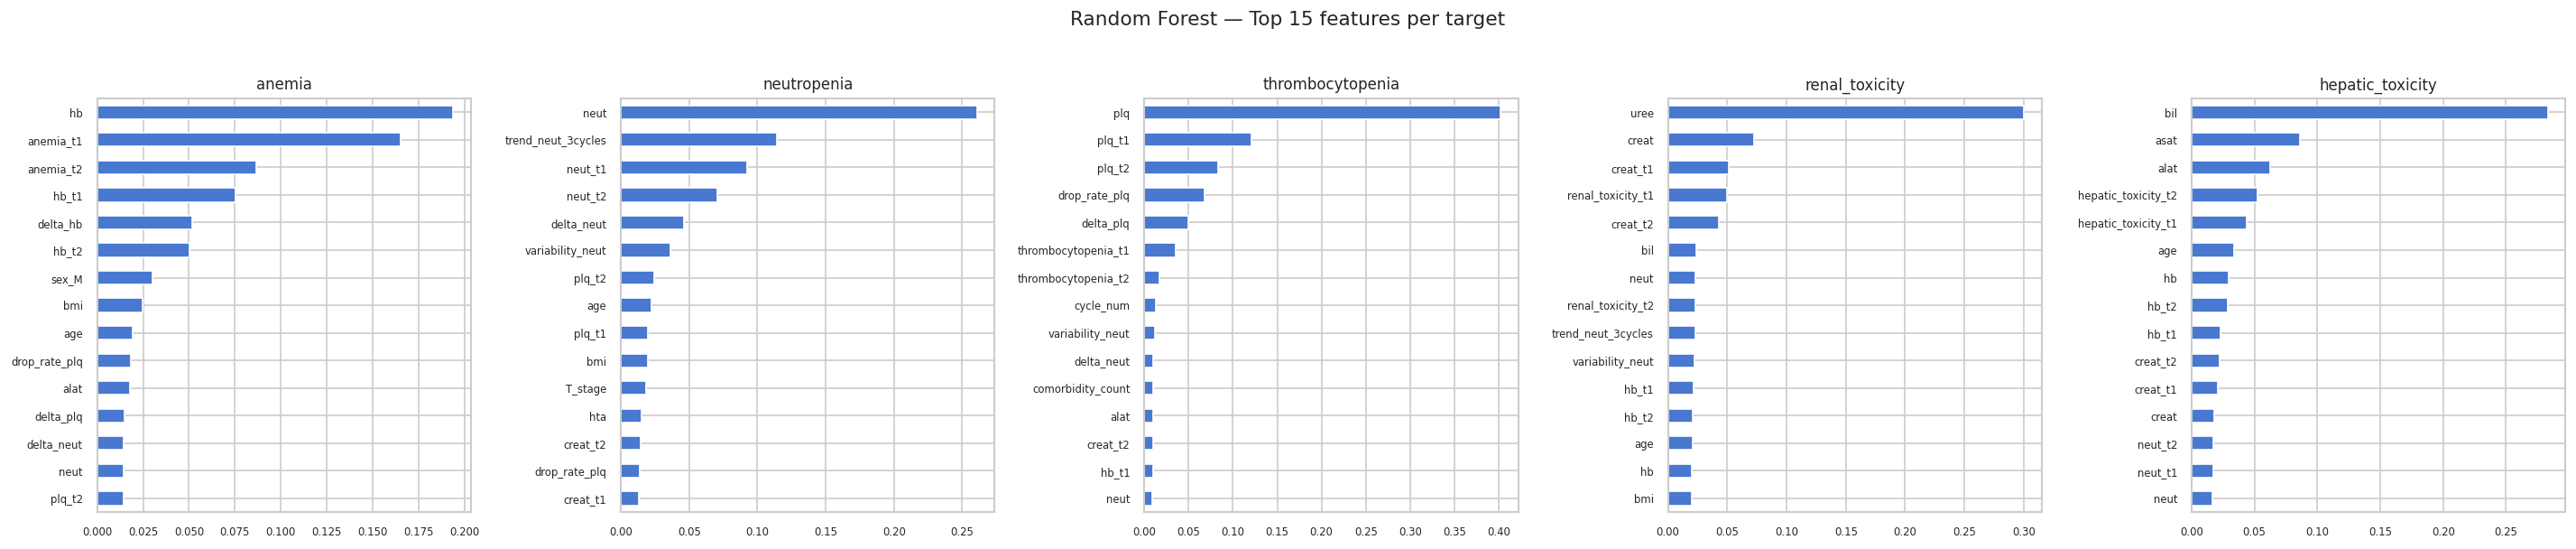
\includegraphics[width=\linewidth]{../outputs/feature_importance_longitudinal.png}
\caption{Diminution Moyenne de l'Impureté (DMI) du Random Forest -- 15 variables les plus importantes par cible de complication, entraîné sur l'ensemble complet d'entraînement.}
\label{fig:fi}
\end{figure}

L'analyse d'importance des variables de la figure~\ref{fig:fi} révèle un schéma cohérent sur les cinq cibles : les \textbf{indicateurs de complications antérieures} (\texttt{anemia\_t1}, \texttt{neutropenia\_t1}, \texttt{hepatic\_toxicity\_t1}) et les \textbf{biomarqueurs décalés} (\texttt{hb\_t1}, \texttt{neut\_t1}, \texttt{plq\_t1}) dominent les classements. Cela valide l'hypothèse centrale du projet : ce qui s'est passé lors du cycle précédent est le meilleur prédicteur de ce qui se passera lors du cycle actuel.

Les variables delta (\texttt{delta\_hb}, \texttt{delta\_neut}) apparaissent dans les premiers rangs pour les cibles correspondantes, confirmant que la direction et la vitesse du changement apportent une valeur prédictive supplémentaire au-delà de la valeur décalée absolue.

Les variables démographiques et de stadification (âge, T\_stage, N\_stage) contribuent moins que l'historique biologique pour toutes les cibles, suggérant que les dynamiques temporelles intra-patient sont plus informatives que les caractéristiques statiques inter-patients pour prédire les complications à court terme.

\section{Prédictions par patient}

Le fichier \texttt{outputs/per\_patient\_predictions.csv} contient, pour chacun des 141 cycles de l'ensemble de test, le résultat réel et la probabilité prédite par l'ensemble pour les cinq complications. Ce tableau permet à l'encadrant clinique de vérifier la plausibilité du modèle sur des patients individuels.

\begin{table}[H]
\centering
\caption{Exemples de lignes du tableau de prédictions par patient (ensemble de test)}
\label{tab:predictions}
\setlength{\tabcolsep}{3pt}
\begin{tabular}{llccccc}
\toprule
\textbf{Patient} & \textbf{Cure} & \textbf{P(Anémie)} & \textbf{P(Neutr.)} & \textbf{P(Thrombo.)} & \textbf{P(Rénale)} & \textbf{P(Hépatique)} \\
\midrule
P1  & 2 & 0,987\,\checkmark & 0,013 & 0,012 & 0,009 & 0,045 \\
P1  & 3 & 0,989\,\checkmark & 0,017 & 0,032 & 0,015 & 0,055 \\
P1  & 4 & 0,987\,\checkmark & 0,019 & 0,874\,\checkmark & 0,015 & 0,034 \\
P108 & 2 & 0,182 & 0,008 & 0,009 & 0,005 & \textbf{0,875}\,\checkmark \\
P108 & 3 & 0,147 & 0,016 & 0,014 & 0,008 & \textbf{0,943}\,\checkmark \\
\bottomrule
\multicolumn{7}{l}{\small \checkmark = vrai positif (complication survenue). Gras = probabilité élevée signalée.}
\end{tabular}
\end{table}

% ══════════════════════════════════════════════════════════════════════════════
\chapter{Discussion}
\label{chap:discussion}
% ══════════════════════════════════════════════════════════════════════════════

\section{Pourquoi les variables longitudinales fonctionnent-elles ?}

Les prédicteurs dominants sur les cinq complications sont les indicateurs de complications antérieures et les biomarqueurs décalés---pas les valeurs du cycle actuel ni les caractéristiques statiques du patient. C'est cliniquement intuitif : un patient qui a eu une anémie lors du cycle précédent a très probablement une anémie à nouveau ; un patient dont les neutrophiles chutent régulièrement est à risque élevé de neutropénie.

Les variables delta et de tendance ajoutent une deuxième couche de signal : elles encodent la \emph{vitesse} et le \emph{momentum} du changement biologique. Une hémoglobine actuelle de 11\,g/dL est interprétée très différemment selon qu'elle a chuté de 2\,g/dL par rapport au cycle précédent (\texttt{delta\_hb}\,=\,-2) ou qu'elle est stable à 11 depuis trois cycles.

\section{Implications cliniques}

\subsection{Pour les complications à forte prévalence (Anémie, Toxicité hépatique)}
Le modèle atteint une sensibilité quasi parfaite (100\,\% et 95,5\,\% respectivement) avec très peu de faux positifs. Ces deux complications représentent la majorité de la charge clinique (68\,\% et 28,6\,\% de prévalence). Le modèle est directement exploitable pour ces cibles : une forte probabilité prédite devrait inciter l'oncologue à envisager un soutien hématopoïétique ou une surveillance de la fonction hépatique avant la prochaine cure.

\subsection{Pour les complications rares (Neutropénie, Toxicité rénale)}
La sensibilité pour la neutropénie est de 50\,\% au seuil de 0,50. Cependant, lorsque le modèle signale un cycle comme neutropénique, il a toujours raison (VPP\,=\,100\,\%). Abaisser le seuil augmenterait la sensibilité au prix de fausses alarmes. L'AUC de 0,954 indique que la discrimination sous-jacente est forte, et le seuil devrait être ajusté dans un contexte prospectif guidé par le coût clinique d'une neutropénie manquée par rapport à une prescription inutile de G-CSF.

La toxicité rénale présente la meilleure discrimination (AUC\,=\,0,999) avec seulement 1 événement manqué. Le modèle peut être utilisé avec une grande confiance pour la surveillance rénale.

\subsection{Protocole clinique proposé}

\begin{enumerate}
  \item \textbf{Cures 1 et 2 :} aucune prédiction disponible (historique insuffisant). La surveillance clinique standard s'applique.
  \item \textbf{Cure $\geq$ 3 :} avant l'administration de la cure, saisir les biomarqueurs actuels du patient et la dose dans le système de prédiction. La sortie est une probabilité pour chacune des cinq complications.
  \item \textbf{Seuils d'action} (suggérés, en attente de validation prospective) :
    \begin{itemize}
      \item $\hat{p} \geq 0{,}50$ : signalement pour discussion ; envisager un ajustement de dose ou un traitement prophylactique.
      \item $\hat{p} \geq 0{,}80$ : signalement fort ; recommander une surveillance renforcée ou un traitement de soutien.
    \end{itemize}
\end{enumerate}

\section{Limites}

\subsection{Taille de l'échantillon}
La cohorte de 108 patients est petite, particulièrement pour les événements rares. Avec seulement 36 cycles neutropéniques dans l'ensemble complet des données et $\approx$4 dans l'ensemble de test, l'estimation de performance pour la neutropénie présente une variance élevée. Les intervalles de confiance sur les métriques de l'ensemble de test seraient très larges.

\subsection{Conception rétrospective monocentrique}
Toutes les données proviennent d'un seul hôpital. Le modèle peut sur-ajuster aux pratiques spécifiques du centre (préparation des médicaments, instruments de mesure, définitions des seuils) et ne pas se généraliser à d'autres centres sans réentraînement. L'évaluation prospective dans un centre indépendant est l'étape essentielle suivante.

\subsection{Sévérité non modélisée}
Les cibles sont binaires (présent/absent). Les complications du FOLFOX vont du grade I (léger, aucune action requise) au grade IV (mettant en danger la vie, nécessitant une hospitalisation). Le modèle actuel ne distingue pas la sévérité, ce qui limite son utilité clinique pour les décisions de gestion des doses.

\subsection{Valeurs de créatinine suspectes}
Environ 20 lignes ont des valeurs de créatinine supérieures à 13\,mg/L pouvant représenter des erreurs d'unité (µmol/L saisi au lieu de mg/L). Celles-ci ont été conservées en attente de confirmation clinique mais peuvent introduire du bruit dans la cible de toxicité rénale.

\subsection{Historique manquant pour les cures 1 et 2}
Le modèle longitudinal ne peut pas être appliqué aux deux premières cures du traitement d'un patient. Pour un schéma de 12 cures, cela signifie que 17\,\% de toutes les cures ne sont pas couvertes.

\section{Perspectives}

\begin{itemize}
  \item \textbf{Validation externe :} collecter des données d'un second centre et évaluer le modèle entraîné sans réentraînement.
  \item \textbf{Prédiction de la sévérité :} reformuler en classification ordinale (grade 0--IV) ou multi-classes.
  \item \textbf{Optimisation du seuil :} utiliser la statistique J de Youden pour sélectionner le seuil optimal par complication basé sur une pondération du coût clinique.
  \item \textbf{Intégration dans le système d'information hospitalier :} connecter le modèle au système d'information du laboratoire pour des prédictions en temps réel à mesure que les résultats biologiques arrivent.
  \item \textbf{Essai prospectif :} randomiser les patients entre une gestion guidée par le modèle et une gestion standard et mesurer les différences de résultats (taux de réduction de dose, taux d'hospitalisation, scores de qualité de vie).
  \item \textbf{Modèles de séquences :} avec un jeu de données plus grand, les architectures LSTM ou Transformer pourraient capturer des patterns temporels plus complexes que l'approche d'ingénierie explicite des variables.
\end{itemize}

% ══════════════════════════════════════════════════════════════════════════════
\chapter{Conclusion}
\label{chap:conclusion}
% ══════════════════════════════════════════════════════════════════════════════

Ce projet démontre qu'un jeu de données rétrospectif modeste de 108 patients sous chimiothérapie FOLFOX, combiné à une ingénierie soigneuse des variables longitudinales et à une méthodologie d'ensemble sans fuite de données, est suffisant pour construire un système prédictif des complications biologiques cliniquement convaincant.

Le résultat central est que \textbf{l'historique des complications antérieures et les biomarqueurs décalés sont les prédicteurs dominants}---pas les données démographiques statiques ni le bilan biologique actuel seul. Cela valide l'approche longitudinale et motive l'encodage explicite de la trajectoire du patient sous forme de variables numériques concrètes.

L'ensemble résultant (XGBoost + LightGBM + Random Forest, vote souple) atteint une \textbf{AUC-ROC moyenne de 0,983} sur cinq complications sur 22 patients non vus. Pour les complications cliniquement critiques, le modèle atteint une sensibilité parfaite ou quasi parfaite : anémie (100\,\%), thrombocytopénie (100\,\%), toxicité hépatique (95,5\,\%) et toxicité rénale (90,9\,\%). La neutropénie, l'événement le plus rare et le plus dangereux, atteint une AUC\,=\,0,954 avec une VPP parfaite---chaque alarme levée pour la neutropénie correspond à un événement réel.

L'ensemble du code, des données (anonymisées), des modèles entraînés et de la documentation est fourni dans les livrables du projet, rendant le système entièrement reproductible et prêt pour une validation prospective.

% ══════════════════════════════════════════════════════════════════════════════
%  RÉFÉRENCES
% ══════════════════════════════════════════════════════════════════════════════
\chapter*{Références}
\addcontentsline{toc}{chapter}{Références}

\begin{enumerate}[label={[\arabic*]}]
  \item André T, Boni C, Mounedji-Boudiaf L, et al. Oxaliplatin, fluorouracil, and leucovorin as adjuvant treatment for colon cancer. \textit{N Engl J Med.} 2004;350(23):2343--2351.
  \item Cassidy J, Clarke S, Díaz-Rubio E, et al. Randomized phase III study of capecitabine plus oxaliplatin compared with fluorouracil/folinic acid plus oxaliplatin as first-line therapy for metastatic colorectal cancer. \textit{J Clin Oncol.} 2008;26(12):2006--2012.
  \item Critères de terminologie communs pour les événements indésirables (CTCAE) v5.0. Institut National du Cancer, 2017.
  \item Breiman L. Random forests. \textit{Mach Learn.} 2001;45(1):5--32.
  \item Chen T, Guestrin C. XGBoost: A scalable tree boosting system. \textit{KDD 2016.} 785--794.
  \item Ke G, Meng Q, Finley T, et al. LightGBM: A highly efficient gradient boosting decision tree. \textit{NeurIPS 2017.}
  \item Pedregosa F, et al. Scikit-learn: Machine learning in Python. \textit{JMLR.} 2011;12:2825--2830.
  \item Strobl C, Boulesteix AL, Zeileis A, Hothorn T. Bias in random forest variable importance measures. \textit{BMC Bioinformatics.} 2007;8:25.
\end{enumerate}

% ══════════════════════════════════════════════════════════════════════════════
%  ANNEXES
% ══════════════════════════════════════════════════════════════════════════════
\appendix

\chapter{Dictionnaire des données}
\label{app:dict}

Le dictionnaire de données complet pour \texttt{dataset\_longitudinal.csv} (704 lignes $\times$ 59 colonnes) est reproduit ci-dessous sous forme résumée. Pour la version complète, voir \texttt{data/data\_dictionary.md}.

\begin{longtable}{p{3.5cm}p{1.5cm}p{2.5cm}p{5.5cm}}
\caption{Résumé du dictionnaire de données} \label{tab:dict} \\
\toprule
\textbf{Colonne} & \textbf{Type} & \textbf{Unité / Valeurs} & \textbf{Description} \\
\midrule
\endfirsthead
\toprule \textbf{Colonne} & \textbf{Type} & \textbf{Unité / Valeurs} & \textbf{Description} \\ \midrule
\endhead
\midrule \multicolumn{4}{r}{\small Suite page suivante} \\
\endfoot
\bottomrule
\endlastfoot
patient\_id & chaîne & P1\ldots P109 & Identifiant patient (non utilisé comme variable) \\
cycle\_num & entier & 0--17 & Numéro de cure ($\geq$2 dans ce jeu de données) \\
age & entier & années & Âge à la première cure \\
sex\_M & binaire & 0/1 & 1 = masculin \\
bmi & flottant & kg/m² & Indice de masse corporelle \\
etat & catégorie & 0/1/2 & Statut nutritionnel (ordinal) \\
hta & binaire & 0/1 & Hypertension artérielle \\
diabetes & binaire & 0/1 & Diabète \\
renal\_disease & binaire & 0/1 & Maladie rénale chronique \\
hepatic\_disease & binaire & 0/1 & Maladie hépatique chronique \\
comorbidity\_count & entier & 0--4 & Somme des quatre comorbidités \\
cancer\_type & catégorie & Colon/\ldots & Localisation tumorale \\
T\_stage & entier & 0--4 & Stade T (TNM) \\
N\_stage & entier & 0--4 & Stade N (TNM) \\
M\_stage & entier & 0--1 & Stade M (TNM) \\
has\_metastasis & binaire & 0/1 & Maladie métastatique \\
treatment\_intent & catégorie & Adj/Neoadj & Intention du traitement \\
interval\_days & entier & jours & Jours depuis la cure précédente \\
dose\_oxali & flottant & mg/m² & Dose d'Oxaliplatine \\
dose\_5fu\_bolus & flottant & mg/m² & Dose de 5-FU bolus \\
dose\_5fu\_cont & flottant & mg/m² & Dose de 5-FU en perfusion continue \\
dose\_af & flottant & mg/m² & Dose d'acide folinique \\
hb & flottant & g/dL & Hémoglobine (actuelle) \\
neut & flottant & G/L & Neutrophiles (actuels) \\
plq & flottant & G/L & Plaquettes (actuelles) \\
uree & flottant & g/L & Urée \\
creat & flottant & mg/L & Créatinine \\
asat & flottant & UI/L & ASAT \\
alat & flottant & UI/L & ALAT \\
bil & flottant & mg/L & Bilirubine totale \\
hb\_t1/t2 & flottant & g/dL & Hb un/deux cycles auparavant \\
neut\_t1/t2 & flottant & G/L & Neutrophiles un/deux cycles auparavant \\
plq\_t1/t2 & flottant & G/L & Plaquettes un/deux cycles auparavant \\
creat\_t1/t2 & flottant & mg/L & Créatinine un/deux cycles auparavant \\
anemia\_t1/t2 & binaire & 0/1 & Anémie survenue à t-1/t-2 \\
neutropenia\_t1/t2 & binaire & 0/1 & Neutropénie à t-1/t-2 \\
thrombocyt.\_t1/t2 & binaire & 0/1 & Thrombocytopénie à t-1/t-2 \\
renal\_tox.\_t1/t2 & binaire & 0/1 & Toxicité rénale à t-1/t-2 \\
hepatic\_tox.\_t1/t2 & binaire & 0/1 & Toxicité hépatique à t-1/t-2 \\
delta\_hb & flottant & g/dL & $\texttt{hb} - \texttt{hb\_t1}$ \\
delta\_neut & flottant & G/L & $\texttt{neut} - \texttt{neut\_t1}$ \\
delta\_plq & flottant & G/L & $\texttt{plq} - \texttt{plq\_t1}$ \\
trend\_neut\_3cycles & flottant & G/L & Moyenne sur 3 cycles des neutrophiles \\
drop\_rate\_plq & flottant & ratio & $(plq - plq_{t2}) / plq_{t2}$ \\
variability\_neut & flottant & G/L & Écart-type sur 3 cycles des neutrophiles \\
target\_anemia & binaire & 0/1 & \textbf{Cible} : anémie cette cure \\
target\_neutropenia & binaire & 0/1 & \textbf{Cible} : neutropénie cette cure \\
target\_thrombocyt. & binaire & 0/1 & \textbf{Cible} : thrombocytopénie \\
target\_renal\_tox. & binaire & 0/1 & \textbf{Cible} : toxicité rénale \\
target\_hepatic\_tox. & binaire & 0/1 & \textbf{Cible} : toxicité hépatique \\
\end{longtable}

\chapter{Reproductibilité}
\label{app:repro}

\section{Environnement logiciel}

\begin{lstlisting}
Python         3.12
pandas         >= 2.0
numpy          >= 1.24
scikit-learn   >= 1.3
xgboost        >= 2.0
lightgbm       >= 4.0
joblib         >= 1.3
matplotlib     >= 3.7
seaborn        >= 0.12
jupyter        >= 1.0
nbconvert      >= 7.0
\end{lstlisting}

\section{Exécution du pipeline}

\begin{lstlisting}[language=bash]
# Installation des dependances
pip install -r requirements.txt

# Etape 1 : Construction du jeu de donnees longitudinal
jupyter nbconvert --to notebook --execute --inplace \
  notebooks/1_data_preparation.ipynb

# Etape 2 : Entrainement et evaluation du modele
jupyter nbconvert --to notebook --execute --inplace \
  notebooks/2_model_longitudinal.ipynb
\end{lstlisting}

Les deux notebooks sont entièrement autonomes et reproduiront tous les tableaux et figures de ce rapport.

\chapter{Structure des fichiers du projet}
\label{app:files}

\begin{lstlisting}
oncolab-ai/
|-- data/
|   |-- raw/
|   |   `-- Collect Data Onco Lab AI - Feuille 2.csv
|   |-- dataset_longitudinal.csv      (704 x 59)
|   `-- data_dictionary.md
|-- notebooks/
|   |-- 1_data_preparation.ipynb
|   `-- 2_model_longitudinal.ipynb
|-- models/
|   |-- anemia_LightGBM.pkl
|   |-- anemia_XGBoost.pkl
|   |-- anemia_RandomForest.pkl
|   |   ... (15 fichiers : 3 modeles x 5 cibles)
|-- outputs/
|   |-- feature_importance_longitudinal.png
|   `-- per_patient_predictions.csv
|-- report/
|   |-- report_fr.tex
|   `-- thesis.md
|-- README.md
`-- requirements.txt
\end{lstlisting}

\end{document}
